\documentclass[twoside,a4paper,11pt,answers]{exam}
\title{MV 1}
\date{}
\usepackage{mystyles}


\author{Vérot, M.}
\date{}
\usepackage[export]{adjustbox}
\usepackage{mathpazo}
\usepackage{booktabs}
\usepackage{framed}


\begin{document}
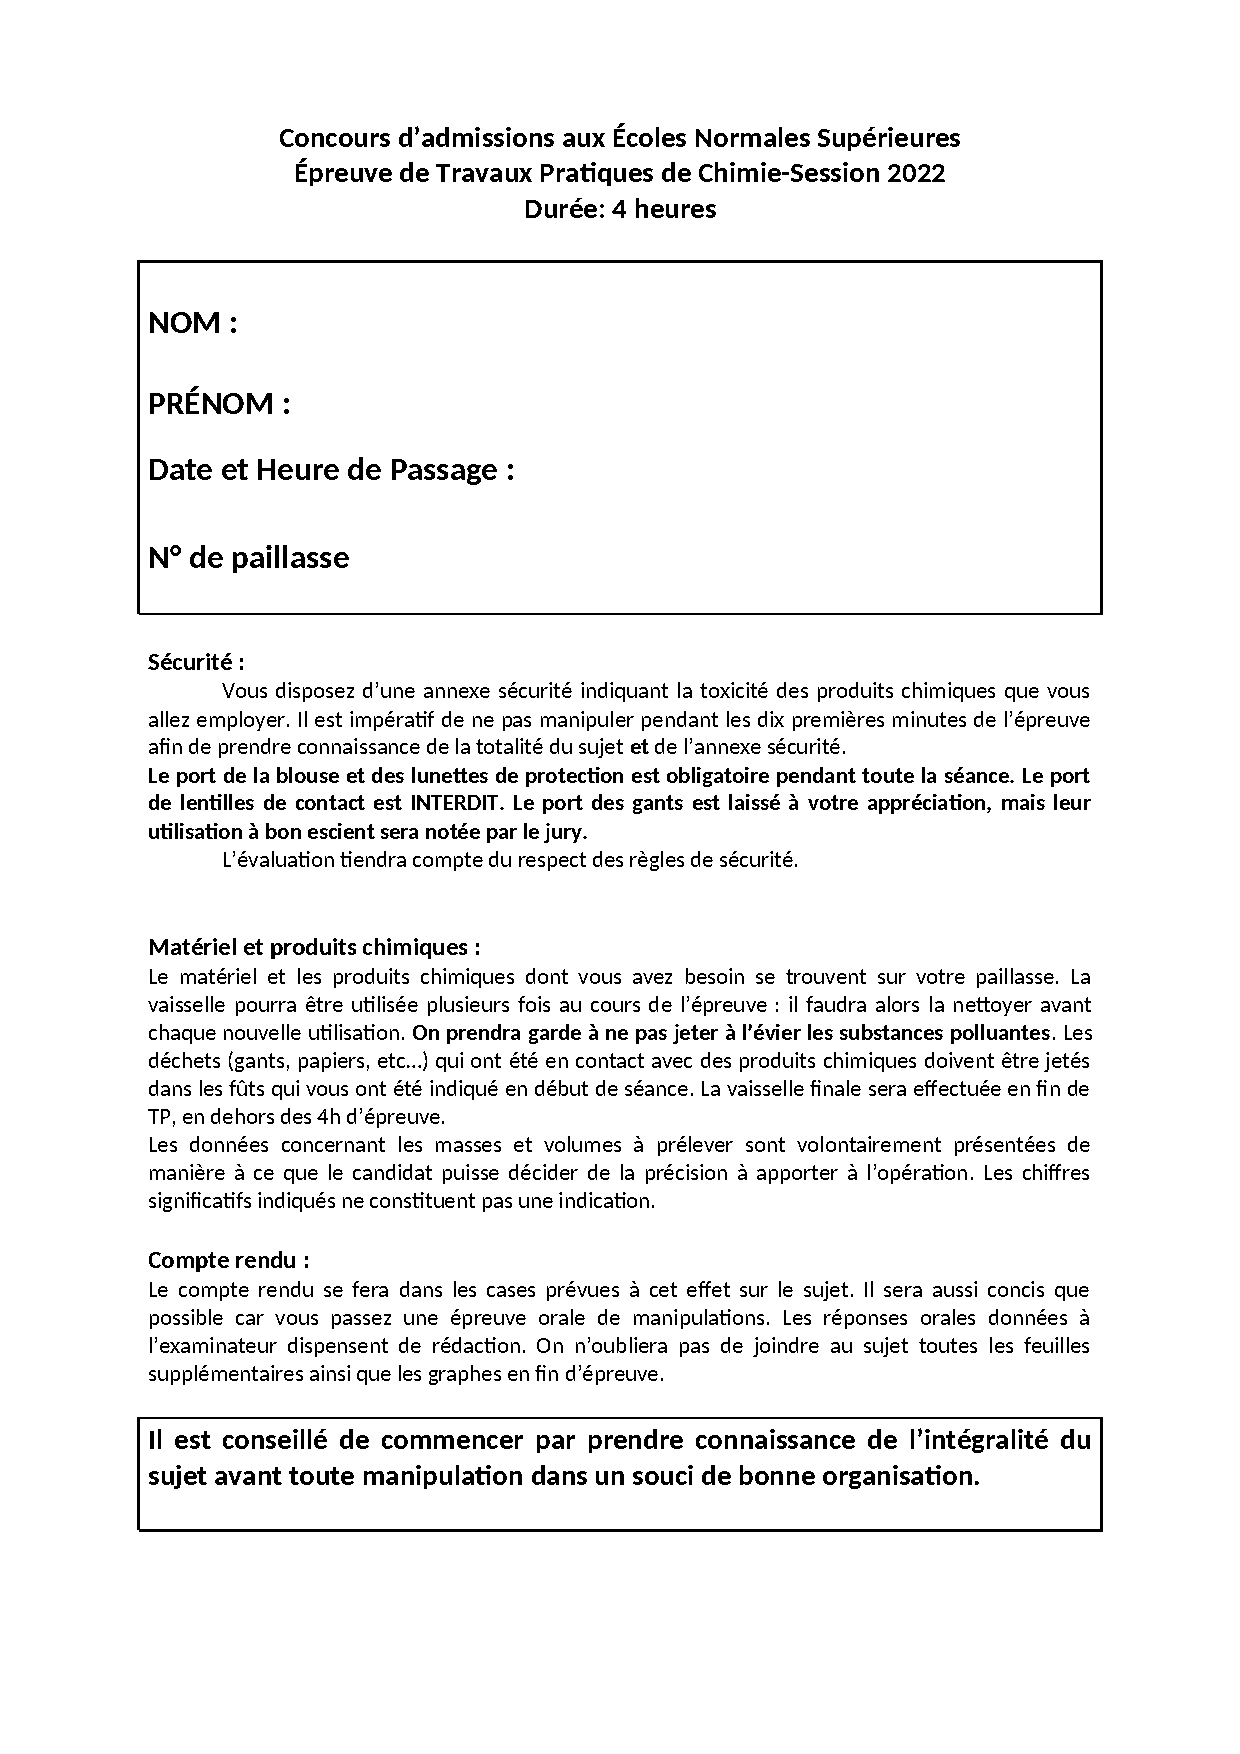
\includepdf[pages = {1}]{page-garde.pdf}

\newpage
%\tito{Les cétones}

Les cétones sont des intermédiaires de synthèse très utilisées en synthèse organique. Avant l'avènement des techniques de spectroscopie modernes, la 2,4-DNPH a été très utilisée pour déterminer la composition des cétones et en particulier leurs masses molaires. Elles peuvent également effectuer de nombreuses réactions comme des étapes de iodation.

\section{Détermination de la masse molaire d'une cétone inconnue}
Nous allons ici nous intéresser à la détermination de la masse molaire d'une cétone grâce à un semi-carbazide, espèce analogue à la 2,4-DNPH mais non explosive à sec.

\bigskip La première étape consiste à synthétiser une semi-carbazone solide à partir du semi-carbazide. Dans un deuxième temps, on effectue l'hydrolyse de la semi-carbazone pour reformer le semi-carbazide initial. Le semi-carbazide formé est alors dosé par une solution de N-bromosuccinimide -- un agent oxydant couramment utilisé en chimie organique.

\subsection{Synthèse de la semi-carbazone}
En présence d'une cétone, le semi-carbazide (figure \ref{fig:carbazone}) permet de former une semi-carbazone solide. Un exemple de formation de semi-carbazone est donné figure \ref{fig:carbazone}.

\begin{figure}[htbp]
 \centering
 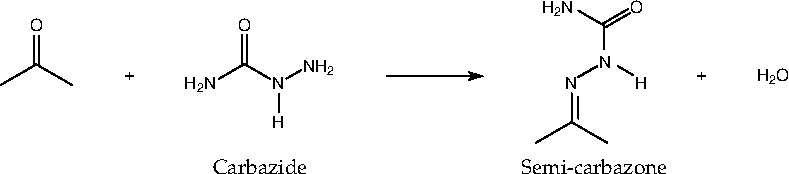
\includegraphics[scale=1]{images/carbazone.pdf}
 \caption{Exemple de formation d'une semi-carbazone si la cétone initiale est l'acétone}
 \label{fig:carbazone}
 \end{figure} 


Prélever 2 g de la cétone inconnue dans un erlenmeyer de 50 mL. Ajouter 10 mL d'eau puis 10 mL d'éthanol. Ajouter ensuite 3 g d'acétate de sodium et 3 g de chlorhydrate de semi-carbazide. Agiter pendant 10 minutes. Filtrer le solide obtenu sur Büchner et laver le solide à l'eau glacée. Recristalliser le solide obtenu en utilisant pour solvant un mélange équivolumique eau/éthanol.

\begin{solution}
Pour la recristallisation, il faut pas mal de solvant (un peu plus de 50 mL) donc ne pas hésiter à les booster pour aller au bout ou engager seulement 1g dans la recristallisation.
\end{solution}

Filtrer et mettre le solide à l'étuve à 100 °C et attendre que la masse soit stable (30 minutes environ). Prendre le point de fusion et faire une CCM de la cétone inconnue et de la semi-carbazone formée en prenant de l'acétate d'éthyle pur comme éluant.

\begin{questions}
\begin{framed}
\question Donner le lien entre la masse molaire de la cétone inconnue notée $M$ et la masse molaire de la semi-carbazone formée.
\begin{solution}[3cm]
La masse molaire du semi-carbazide est égale à : \begin{align}
M\left(\text{semi-carbazide} \right)=3\times 14+5+12+16=75~\ch{g\cdot mol^{-1}}\\
M\left(\text{carbazone} \right)=M+M\left(\text{semi-carbazide} \right)-M(\ch{H_2O})=M+57 ~\ch{g\cdot mol^{-1}}
\end{align}
Ou en partant des masses molaires données en annexe :
\begin{align}
M\left(\text{carbazone} \right)={}&M+M\left(\text{semi-carbazide,HCl} \right)-M(\ch{H_2O})-M(\ch{HCl})\\
={}&M+111,53-18-36,45=M+57~\ch{g\cdot mol^{-1}}
\end{align}
\end{solution}
\end{framed}
\begin{framed}
\question Indiquer le rôle de l'acétate de sodium.
\begin{solution}[3cm]
Il permet d'éviter d'avoir un milieu trop acide (on introduit le chlorhydrate de semi-carbazide, donc HCl) pour garder la nucléophilie de l'azote en formant de l'acide acétique (dont on distingue nettement l'odeur avant recristallisation).
\end{solution}
\end{framed}

\begin{framed}
\question Calculer les rapports frontaux des différents composés et justifier l’ordre d’élution.
\begin{solution}[5cm]
Pour la cétone : 0,77 pour la carbazone : 0,54 (tâche large).

La cétone est polaire non protique alors que la carbazone est polaire protique, l'acétate d'éthyle est polaire protique. 

La carbazone est plus retenue que la cétone (présence de liaisons H).
\end{solution}
\end{framed}
\begin{framed}
\question Donner la température de fusion de la semi-carbazone formée.
\begin{solution}[5cm]
Après recristallisation : 207 à 209 °C (valeur tabulée et mesurée expérimentalement)
\end{solution}
\end{framed}

\begin{framed}
\question Calculer le rendement de la synthèse et commenter la pureté du solide obtenu.
\begin{solution}[5cm]
J'ai obtenu 2,014 g soit un rendement de 68 \%. (le calcul n'est possible qu'après avoir déterminé la masse molaire de la semi-carbazone).

La masse molaire de la semi-carbazone attendue est $177,23~\ch{g\cdot mol^{-1}}$ et il y avait initialement 16,7 mmol d'acétophénone et 26,9 mmol de semi-carbazide et 36,6 mmol d'acétate de sodium.
\end{solution}
\end{framed}

%\newpage

\fullwidth{

\subsection{Titrage de la semi-carbazone}
Le semi-carbazide peut être oxydé par le N-Bromosuccinimide (NBS) pour former de l'acide carbamique. Ce dosage peut être fait en utilisant pour indicateur de fin de réaction le rouge de méthyle. Les deux couples d'oxydo-réduction impliqués sont donnés figure \ref{fig:NBS}.}


\begin{figure}[htbp]
\centering
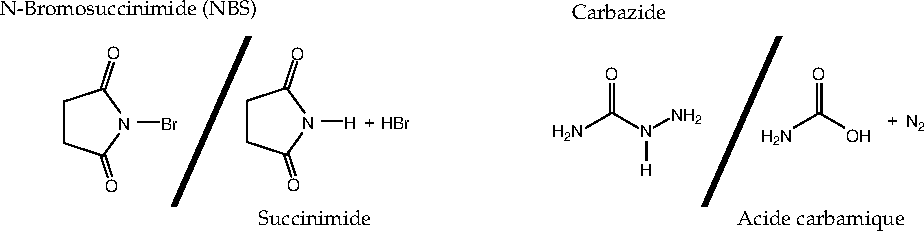
\includegraphics[scale=1]{images/NBS-1.pdf}
\caption{Les deux couples d'oxydo-réduction impliqués lors du dosage.}
\label{fig:NBS}
\end{figure}

\fullwidth{\subsubsection{Étalonnage de la solution de N-bromosuccinimide}
Les solutions de N-bromosuccinimide ne sont pas stables dans le temps et doivent être préalablement étalonnées.

\bigskip
Proposer un protocole pour 
\begin{itemize}
\item étalonner une solution de N-bromosuccinimide à 1 $~\ch{g \cdot L^{-1}}$ par une solution de semi-carbazide à l'aide des produits et du matériel disponible ;
\item montrer également que le rouge de méthyle est un indicateur de fin de réaction adapté pour suivre le dosage.
\end{itemize} 



\textit{Indications} : 
\begin{itemize}
\item On ajoutera 10 mL d'acide sulfurique à 20 \% à la solution permettant de faire l'étalonnage. 
\item L'espèce à titrer pour effectuer l'étalonnage devra être sèche.
\item Préparer 250 mL de solution de N-bromosuccinimide à 1 $~\ch{g \cdot L^{-1}}$.
\item L'équivalence étant plus ou moins difficile à repérer, répéter le dosage jusqu'à avoir deux volumes équivalents concordants (écart de 0,2 mL maximum). 
\item La dissolution du NBS peut être lente, dans ce cas, utiliser la cuve à ultra-son. 
\end{itemize}

\textit{Après validation par un examinateur du protocole, mettre en œuvre la manipulation.}}


\begin{solution}
Il faut calculer la concentration de la solution en N-bromosuccinimide :
\begin{align}
C_{NBS}=\dfrac{m_{NBS}}{M_{NBS}\times V}=\dfrac{250\cdot 10^{-3}}{177,98\times 250\cdot 10^{-3}}=5,62\cdot 10^{-3}~\ch{mol \cdot L^{-1}}
\end{align}

\bigskip

Il faut ensuite trouver l'équation de dosage, on commence par trouver les deux demi-équations rédox :
\begin{align}
\ch{NBS+2~H^{+}+2~e^{-}}={}&\text{\emph{succinimide}}+\ch{HBr}\\
\text{\emph{semi-carbazide}}+\ch{H_2O}={}&\text{\emph{Ac. carbamique}}\ch{+N_2+4~e^{-}+4~H^{+}}
\end{align}
L'équation de dosage est donc :
\begin{center}
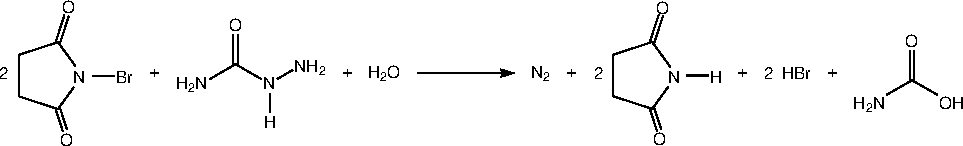
\includegraphics[scale=1]{images/dosage.pdf}
\end{center}
On cherche à avoir un volume équivalent vers 20 mL, soit environ :
\begin{align}
n_{carb}= \dfrac{C_{NBS}V_{eq}}{2} =5,62\cdot 10^{-3}\dfrac{20\cdot 10^{-3}}{2}= 5,62\cdot 10^{-5}~\ch{mol}=6,26~\ch{mg} 
\end{align}
La masse est trop faible pour être pesée directement, on peut donc préparer une solution avec 62,6 mg dans une fiole de 50 mL et en prélever 5 mL. (ou 50 mg dans 50 mL, prélever 5 mL pour un volume équivalent autour de 16 mL).
\bigskip
\textbf{Attention au facteur 2 dans l'équation de dosage.}

Pour montrer que le rouge de méthyle est un bon indicateur de fin de réaction, dans 3 tubes à essai : 
on ajoute : 1 ou deux gouttes de solution de semi-carbazide (tube 1), 3 mL de solution de semi-carbazide (tube 2), rien (tube 3). On égalise les niveaux, on ajoute de l'acide sulfurique à 20 \% (2 mL max), quatre gouttes de rouge de méthyle dans chacun des tubes.

Tous les tubes sont rouges : avant réaction on a une coloration. On ajoute 2 mL de solution de NBS : les tubes 1 et 3 se décolorent mais pas le tube 2 : le NBS oxyde le rouge de méthyle et le semi-carbazide (tube 1 et 3), il commence par oxyder le semi-carbazide avant d'oxyder le rouge de méthyle (tube 2). 

\bigskip
Le dosage demande d'avoir des tubes témoins (cf ci-dessus) car à l'approche de l'équivalence la coloration est rose très pâle. De même, il faut du papier blanc en fond pour distinguer la couleur rose. En cas de souci pour détecter l'équivalence, on peut aller jusqu'à une douzaine de gouttes de rouge de méthyle si nécessaire.
\end{solution}

%\newpage
\fullwidth{\subsubsection{Hydrolyse et titrage de la semi-carbazone inconnue}
Peser environ exactement 70 mg de semi-carbazone recristallisée et séchée, la dissoudre en complétant avec de l'éthanol dans une fiole de 50 mL. Pipeter 5 mL de cette solution dans un ballon de 100 mL et ajouter 10 mL d'acide sulfurique à 20 \%. Porter le mélange à ébullition pendant 30 minutes. Rincer le réfrigérant et les parois du ballon avec un minimum d'eau. Refroidir le ballon à température ambiante et doser la solution dans le ballon en présence de rouge de méthyle avec la solution de N-bromosuccinimide précédemment préparée.}

\begin{framed}
\question Donner l'équation bilan de la réaction ayant lieu lors du reflux et donner le rôle de l'acide sulfurique.
\begin{solution}[3cm]
Il s'agit de l'hydrolyse, c'est donc la réaction inverse de celle donnée \ref{fig:carbazone}. L'acide sulfurique sert ici de catalyseur et permet de rester en milieu acide pour garder la couleur rouge pour l'indicateur coloré.
\end{solution}
\end{framed}

\begin{framed}
\question En déduire la masse molaire de la cétone
\begin{solution}[7cm]
Le volume équivalent est aux alentours de 14 mL donc on en déduit la quantité de semi-carbazide initialement présente dans le milieu :
\begin{align}
n_{carb}=\dfrac{V_{eq}}{2}\times C_{NBS}=\dfrac{14\cdot 10^{-3}}{2}\times 5,62\cdot 10^{-3}=3,93\cdot 10^{-5}~\ch{mol}
\end{align}
La masse initiale était de 70 mg et on en a prélevé un dixième donc 7 mg de semi-carbazone libère $3,93\cdot 10^{-5}~\ch{mol}$ de semi-carbazide. 

On en déduit :
\begin{align}
M_{\text{carbazone}}=\dfrac{m}{n_{carb}}=\dfrac{7\cdot 10^{-3}}{3,93\cdot 10^{-5}}=178,1~\ch{g\cdot mol^{-1}}
\end{align}
La masse molaire de la cétone est donc de 
\begin{align}
M_{\text{cétone}}=178,1-57 = 121,1 ~\ch{g\cdot mol^{-1}}
\end{align}


En pratique, il s'agit de l'acétophénone dont la masse molaire vaut $120,15~\ch{g\cdot mol^{-1}}$. Un calcul d'incertitude permet de voir que le résultat est en accord avec la valeur théorique.
\end{solution}
\end{framed}

\begin{framed}
\question Donner l'intérêt d'être passé par la semi-carbazone et indiquer une/des condition(s) nécessaire(s) pour que cette méthode de détermination de la masse molaire soit juste.
\begin{solution}[3cm]
On a pu former un solide de grande pureté grâce à la recristallisation (première condition nécessaire vérifiée par CCM et point de fusion) (il faut aussi ne pas partir d'un mélange de cétones).

Si l'hydrolyse est quantitative (deuxième hypothèse nécessaire), la quantité de semi-carbazide est alors directement indicative de la quantité de matière dans la solution de carbazone. On a ainsi pu doser la cétone indirectement en dosant le semi-carbazide issu de l'hydrolyse de la carbazone.
\end{solution}
\end{framed}


\fullwidth{\section{Cinétique de l'iodation de la cyclohexanone}

Les cétones peuvent être iodées en présence de diiode. La cinétique globale de la iodation pour la cyclohexanone est relativement complexe mais elle admet un ordre apparent par rapport à différents constituants après un temps d'induction suffisant. La cinétique de réaction sera suivi à 565 nm.

\bigskip
Dissoudre 2,45 g de cyclohexanone dans une fiole jaugée de 50 mL, cette solution sera la solution \textbf{A}. 

Dans un bécher de 50 mL, mélanger 5 mL de la solution \textbf{A}, 5 mL de la solution d'acide chlorhydrique à 0,5 $~\ch{mol \cdot L^{-1}}$ et 13 mL d'eau (solution n° 0, tableau \ref{tab:cin}). Faire le blanc avec cette solution.

}

\begin{table}[htbp]
\centering
\begin{tabular}{lrrrrrrrrrrrr}
\toprule
Essai & 0 & 1 & 2 & 3 \\
\midrule
$V(\mathbf{A})$ & 5 & 5 & 7 & 10 \\
$V\left(\ch{HCl}; 0,5 ~\ch{mol \cdot L^{-1}} \right)$ & 5 & 5 & 5 & 5 \\
$V(\ch{H_2O})$ & 13 & 10 & 7 & 5 \\
$V(\ch{I_3^{-}})$& 0 & 3 & 3 & 3  \\ 
\bottomrule
\end{tabular}
\caption{Suivis cinétiques à réaliser. La solution d'ions triiodure est déjà prête.}
\label{tab:cin}
\end{table}

\fullwidth{Pour chacun des essais, réaliser les différents mélanges en ajoutant la solution de triiodure en dernier. Déclencher le chronomètre lors de l'introduction de la solution de triiodure. Agiter jusqu'à ce que la solution ne soit plus trouble et transvaser dans la cuve de mesure. Noter l'évolution de l'absorbance à 565 nm  pendant une vingtaine de minutes ou jusqu'à disparition de la coloration.

\bigskip
Des expériences analogues en faisant varier la concentration en acide ont permis de montrer que la réaction admet un ordre 1 par rapport à cette espèce.}

\begin{framed}
\question  Calculer les concentrations initiales pour chacun des réactifs. Commenter.
\begin{solution}[6cm]
 \begin{align}
\con{cyclohexanone}_{0}=\dfrac{2,45}{98,14\times 50\cdot 10^{-3}}=0,5 ~\ch{mol \cdot L^{-1}} \qquad \con{I_2}_0=0,05 ~\ch{mol \cdot L^{-1}}
\end{align}

\begin{tabular}{lrrrrrrrrrrrr}
\toprule
Essai & 0 & 1 & 2 & 3 \\
\midrule
$\con{\ch{cyclohexanone}}$ &  & $1,08\cdot 10^{-1}$ & $1,52\cdot 10^{-1}$ & $2,17\cdot 10^{-1}$ \\
$\con{\ch{HCl}}$ &  & $1,08\cdot 10^{-1}$ & $1,08\cdot 10^{-1}$ & $1,08\cdot 10^{-1}$ \\
$\con{I_3^{-}}$&  & $6,52\cdot 10^{-3}$& $6,52\cdot 10^{-3}$ & $6,52\cdot 10^{-3}$  \\ 
\bottomrule
\end{tabular}


On travaille en dégénérescence d'ordre par rapport aux ions triiodure ($\con{I_3^{-}}\ll \con{cyclohexanone},\con{HCl}$).

\end{solution}
\end{framed}
\begin{framed}
\question Une fois les différentes courbes obtenues, montrer qu'il y a deux phases distinctes lors de la cinétique.
\begin{solution}[3cm]
Initialement, il y a un trouble et l'évolution est non linéaire. Cela est d'autant plus visible que la concentration en cyclohexanone est élevée. Celà correspond au temps d'induction avant d'arriver à un régime pseudo-stationnaire

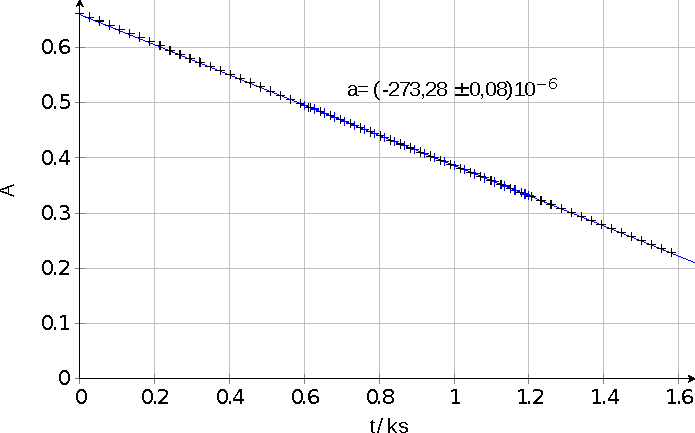
\includegraphics[scale=0.5]{images/curve_1.pdf}

courbe de l'expérience 1, on n'observe pas forcément 2 phases de réaction.

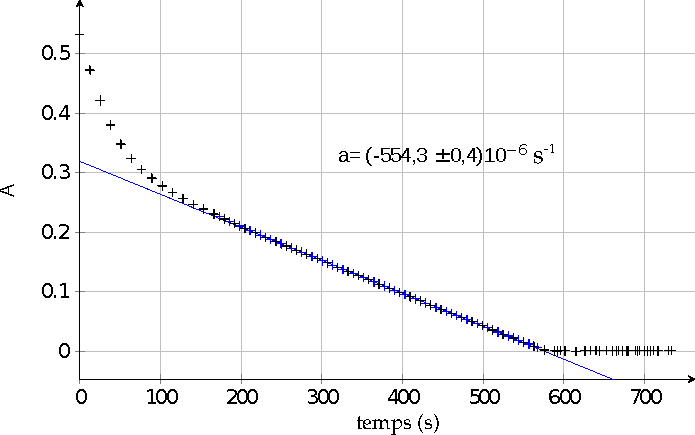
\includegraphics[scale=0.5]{images/curve_2.pdf}

 Courbe de l'expérience 3
\end{solution}
\end{framed}

\begin{framed}
\question Tracer l'évolution de l'absorbance en fonction du temps et donner l'ordre apparent par rapport aux ions triiodure lors de la deuxième phase de la cinétique.
\begin{solution}[3cm]
~

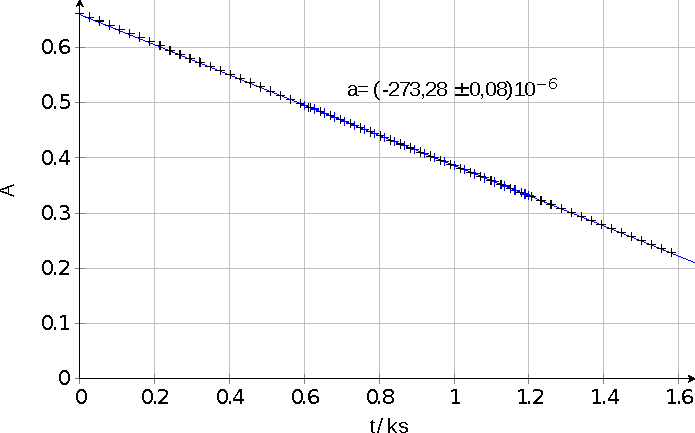
\includegraphics[scale=0.5]{images/curve_1.pdf}

courbe de l'expérience 1

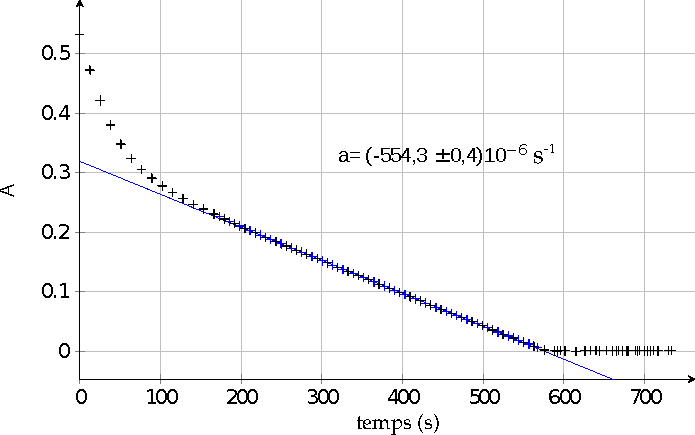
\includegraphics[scale=0.5]{images/curve_2.pdf}

 Courbe de l'expérience 3

Après quelques minutes, la décroissance est quasi linéaire. L'ordre par rapport au diiode est donc 0 (dégénérescence d'ordre).
\end{solution}
\end{framed}
\begin{framed}
\question  À l'aide des différentes expériences, en déduire l'ordre apparent par rapport à la cyclohexanone lors de la deuxième phase de la cinétique.
\begin{solution}[3cm]
Il faut tracer $k_{app}=f(\con{cyclohexanone})$ pour les trois expériences, la constante apparente évolue linéairement donc l'ordre par rapport à la cyclohexanone est 1.

À 25 °C, j'ai eu :
\begin{itemize}
\item $k_{app,1}=273\cdot 10^{-6}~\ch{s^{-1}}$
\item $k_{app,2}=383\cdot 10^{-6}~\ch{s^{-1}}$
\item $k_{app,3}=554\cdot 10^{-6}~\ch{s^{-1}}$
\end{itemize}
\end{solution}
\end{framed}


\begin{framed}
\question  Commenter le choix de la longueur d'onde de suivi.
\begin{solution}[3cm]
À 565 nm, il y a un point isobestique pour les ions triiodure/diiode. On n'est donc pas au maximum d'absorbance mais cela permet de s'affranchir de l'équilibre de complexation pour former les ions triiodure.
\end{solution}
\end{framed}

\begin{framed}
\question Indiquer des conditions nécessaires pour que le mécanisme réactionnel proposé figure \ref{fig:MR} corresponde aux observations expérimentales (vitesse relative des différentes étapes).
\begin{solution}[3cm]
On observe un ordre 1 par rapport à la cyclohexanone et l'acide mais un ordre zéro par rapport aux espèces iodées. Il faut donc que l'étape cinétiquement déterminante soit la deuxième et pas la troisième ni la quatrième. La vitesse de l'étape 2 doit donc être la vitesse limitante (« $v_2\ll v_3 \ll v_4$ » même si la formulation est restrictive ).
\end{solution}
\end{framed}

\end{questions}

\newpage
\section*{Annexe}

\subsection*{Données}



\begin{itemize}
%\item Les températures de fusion des semi-carbazones sont usuellement de l'ordre de 200 °C.
\item Solubilité du N-bromosuccinimide dans l'eau à 25 °C : 14,7 $~\ch{g\cdot L^{-1}}$
\item Solubilité du semi-carbazide dans l'eau à 25 °C : 9,2 $~\ch{g\cdot L^{-1}}$
\item Zone de virage du rouge de méthyle : 4,8 - 6,0
\begin{figure}[htbp]
\centering
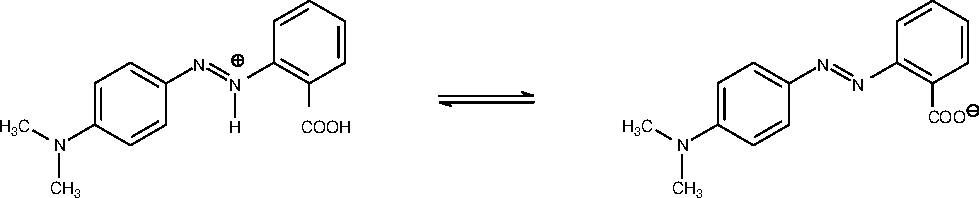
\includegraphics[scale=0.75]{images/Methyl_red.pdf}
\caption{Formes acido-basiques du rouge de méthyle}
\label{fig:rmethyl}
\end{figure}
\item $\ch{I_{2(aq)}+I^{-}_{(aq)}=I_{3(aq)}^{-}}$ \qquad $K=7,1\cdot 10^{2}$

\end{itemize}
\begin{table}[htbp]
\centering
\begin{tabular}{lrrrrrrrrrrrr}
\toprule
&N&C&Cl&H&O\\
\midrule
Masse molaire ($~\ch{g\cdot mol^{-1}}$)&14,01 &12,01&35,45&1,01&16,00\\
\bottomrule
\end{tabular}
\caption{Masse molaire de certains éléments.}
\label{tab:MM}
\end{table}

\noindent\begin{minipage}[t]{0.45\textwidth}
\centering
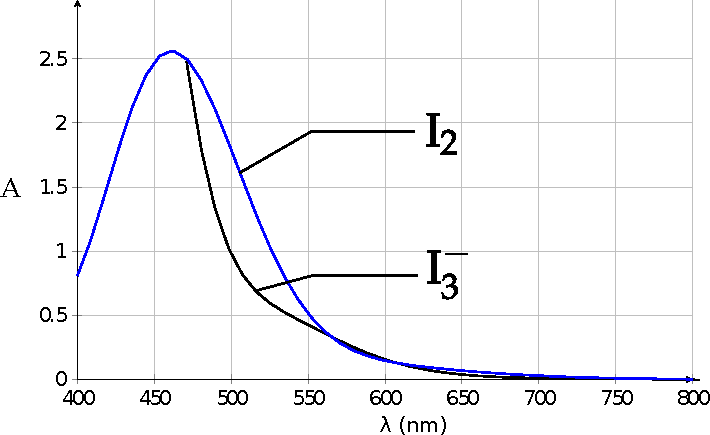
\includegraphics[width=1\textwidth]{images/abs.pdf}
\captionof{figure}{Spectres de solutions de même concentration en diiode et en ions triiodure.}
\label{fig:spectre}
\end{minipage}\begin{minipage}[t]{0.45\textwidth}
\begin{flushright}
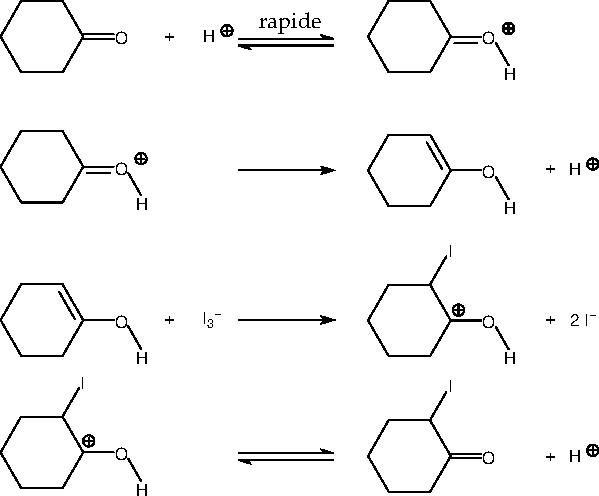
\includegraphics[scale=0.7]{images/MR.pdf}
\end{flushright}
\captionof{figure}{Mécanisme réactionnel proposé.}
\label{fig:MR}
\end{minipage}







\newpage
\subsection*{Précautions et risques associés aux produits chimiques utilisés}

\noindent\begin{tabular}{p{6.7cm}p{2cm}p{7cm}rrrrrrrrrr}
\toprule
Produit & Sécurité & Risque (H) Prudence (P) \\
\midrule
Semicarbazide, chlorhydrate\newline (563-41-7, 111,53 g/mol) & 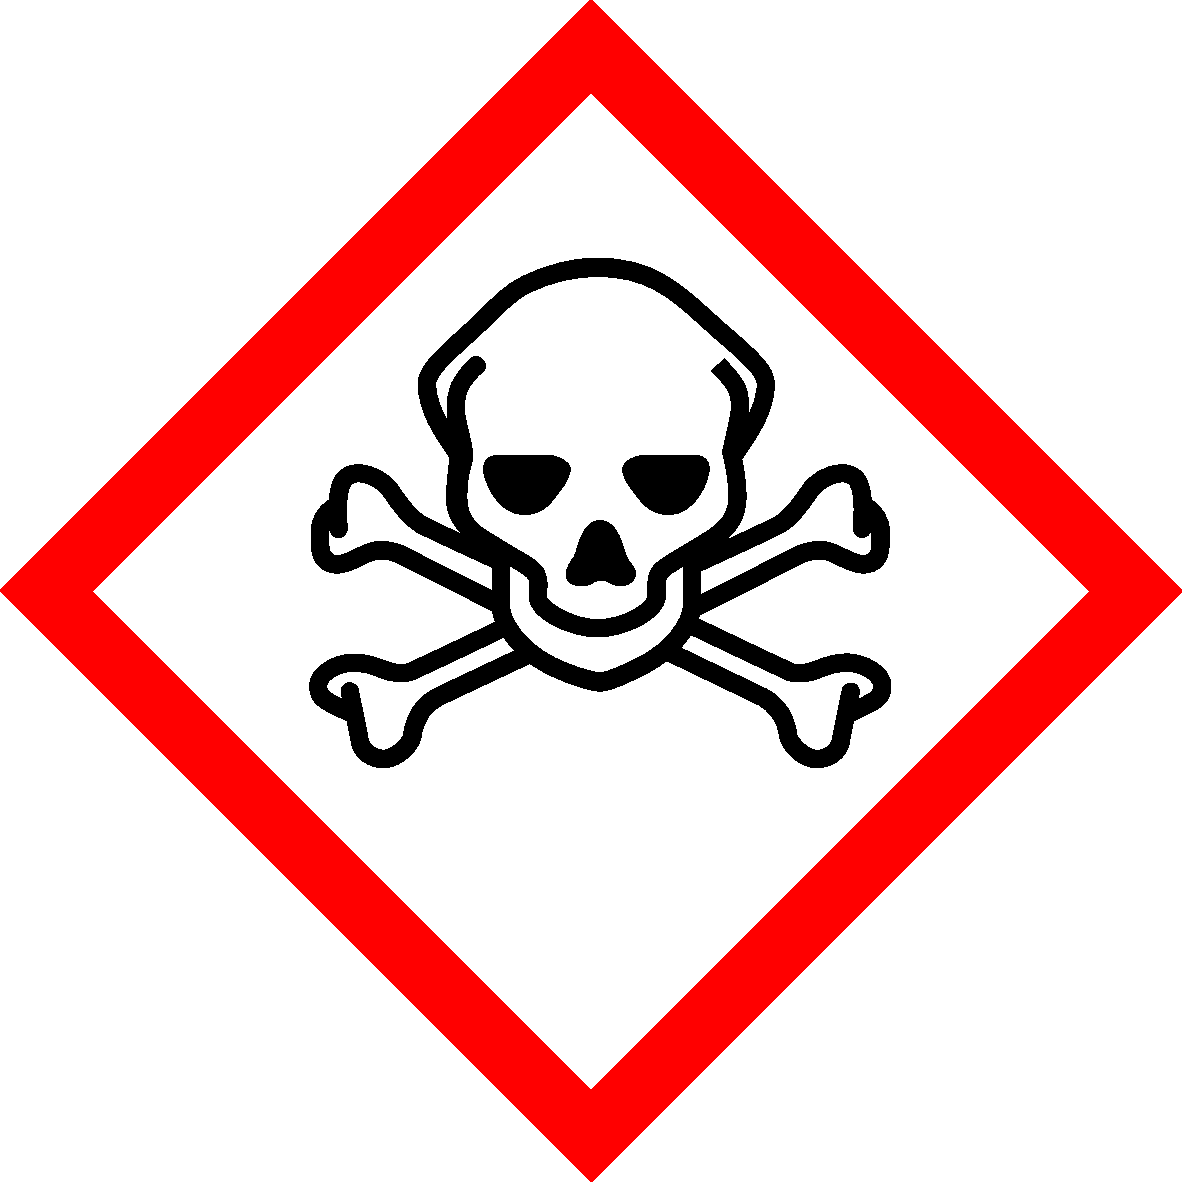
\includegraphics[height=24pt,valign=t]{pictos/toxic.pdf} &  
H301\newline P301 + P310\\
\midrule
Acétate de sodium\newline (127-09-3, 82,03 g/mol) &  &   \\
\midrule
N-Bromosuccinimide\newline (128-08-5, 177,98 g/mol) & 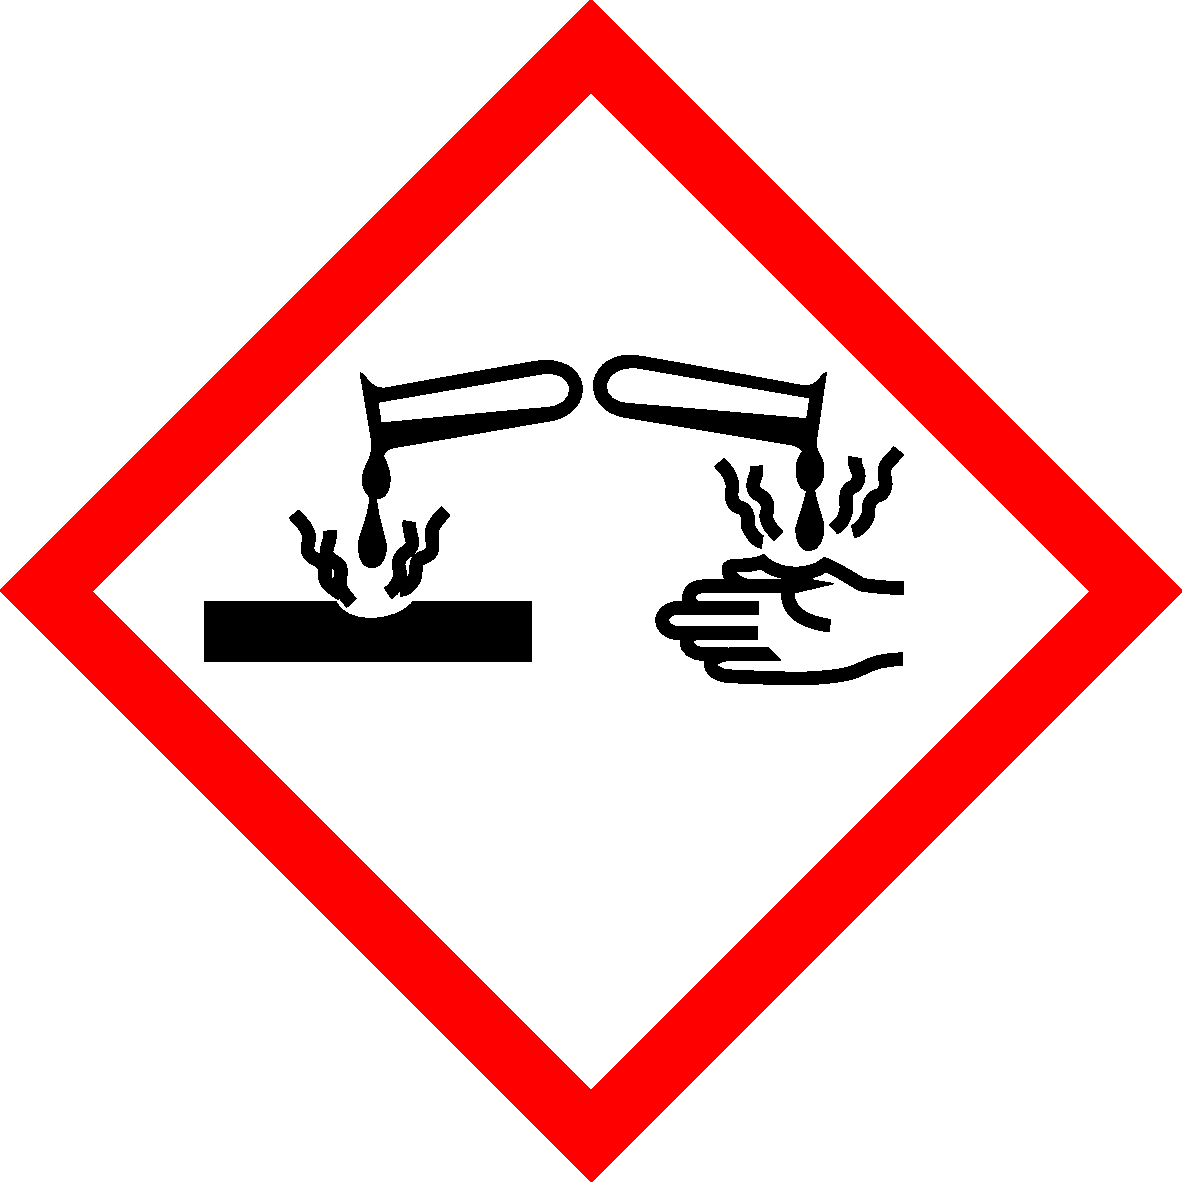
\includegraphics[height=24pt,valign=t]{pictos/corro.pdf} 
\includegraphics[height=24pt,valign=t]{pictos/exclam.pdf}&  
H302, H314\newline P280, P305 + P351 + P338, P310\\
\midrule
Acétophénone\newline (98-86-2, 120,15 g/mol) & 
\includegraphics[height=24pt,valign=t]{pictos/exclam.pdf} &  
H302, H319\newline P305 + P351 + P338\\
\midrule
Cyclohexanone\newline (108-94-1, 98,14 g/mol) & 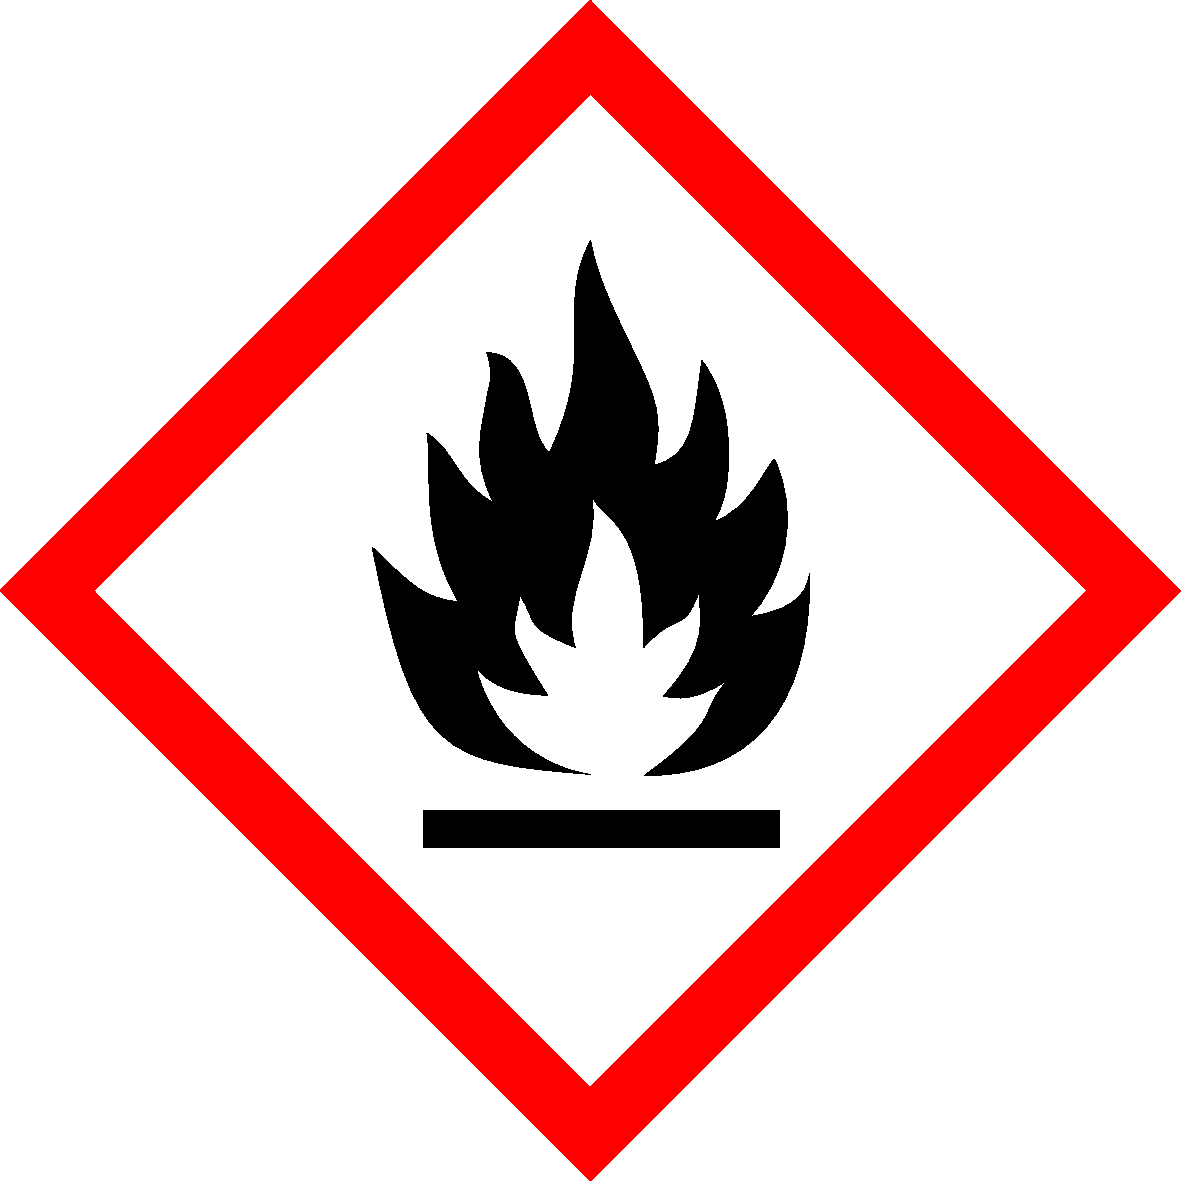
\includegraphics[height=24pt,valign=t]{pictos/flamm.pdf}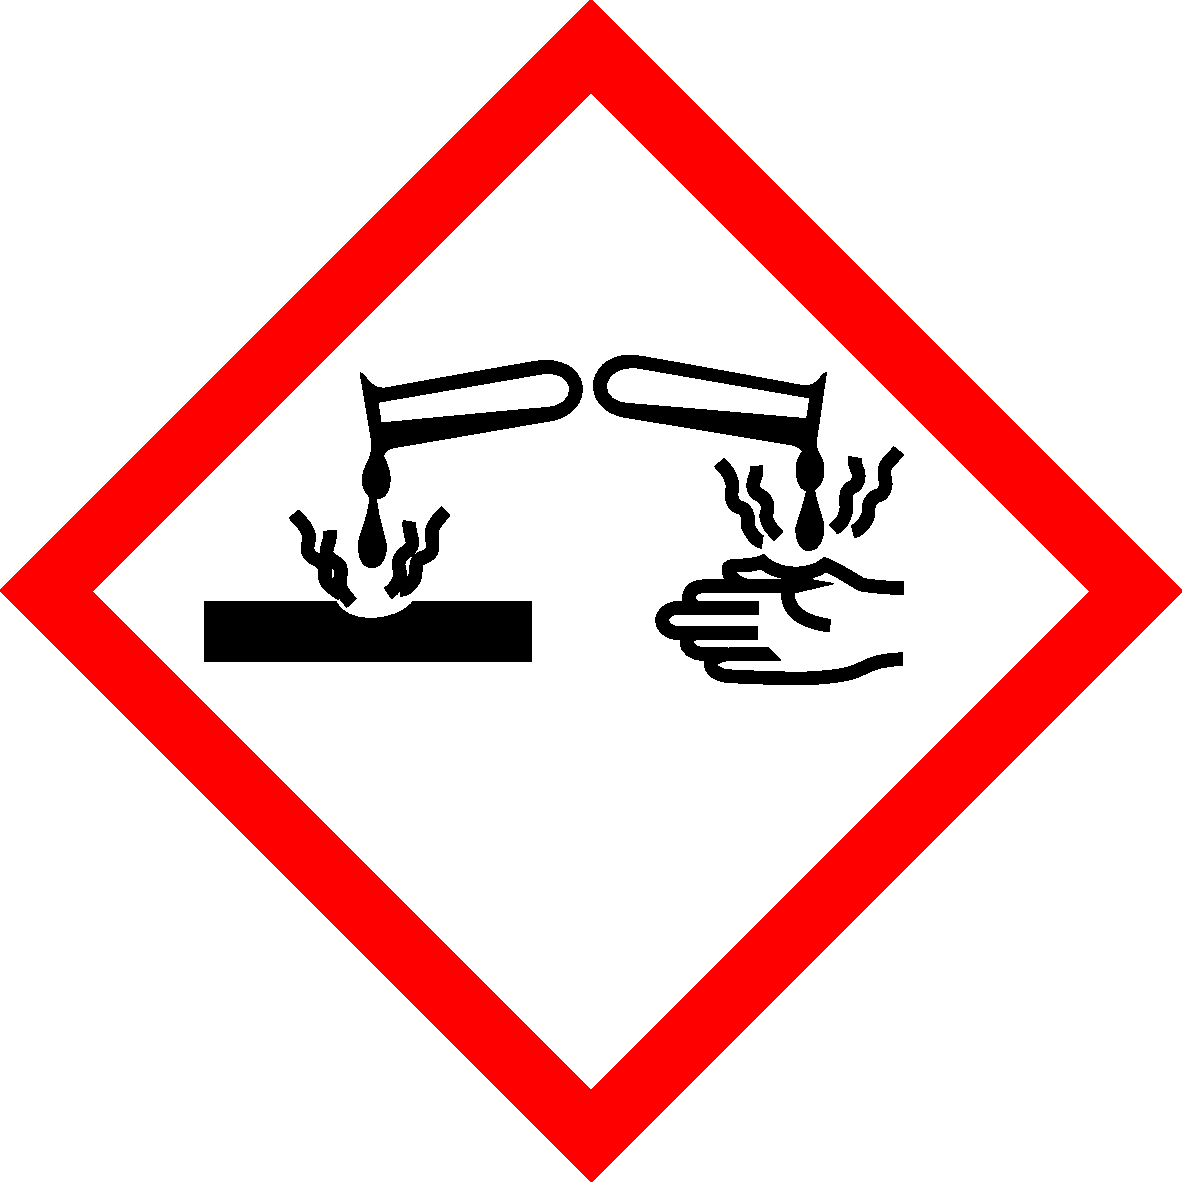
\includegraphics[height=24pt,valign=t]{pictos/corro.pdf} 
\includegraphics[height=24pt,valign=t]{pictos/exclam.pdf} &  
H226, H302, H315, H318\newline P280, P305 + P351 + P338\\
\midrule
Diiode\newline (7553-56-2, 253,81 g/mol) & 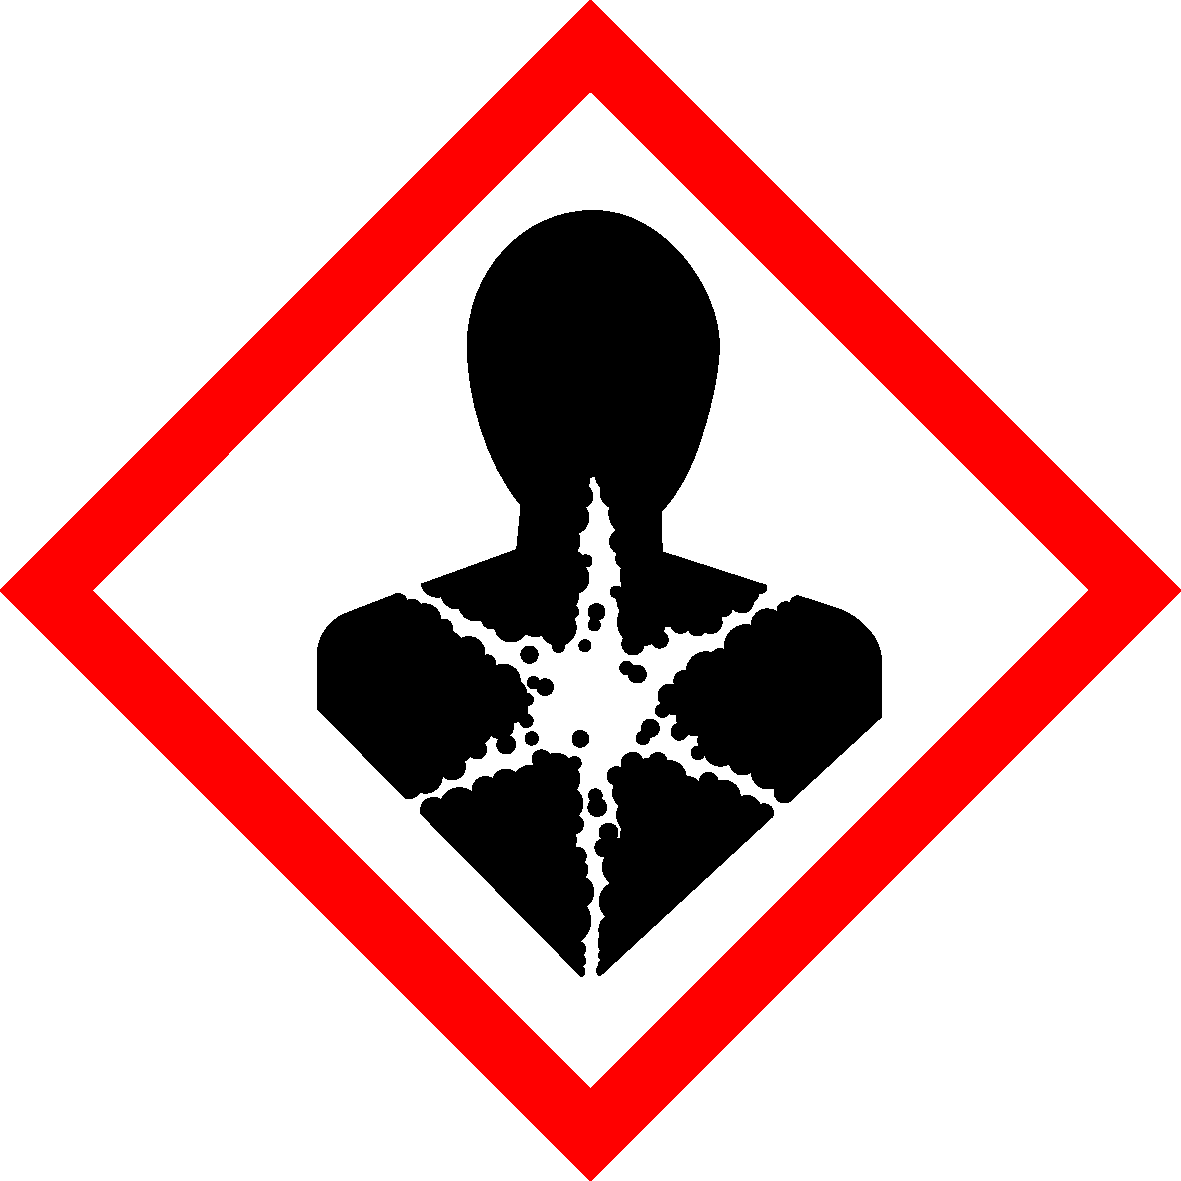
\includegraphics[height=24pt,valign=t]{pictos/cmr.pdf}
\includegraphics[height=24pt,valign=t]{pictos/exclam.pdf} 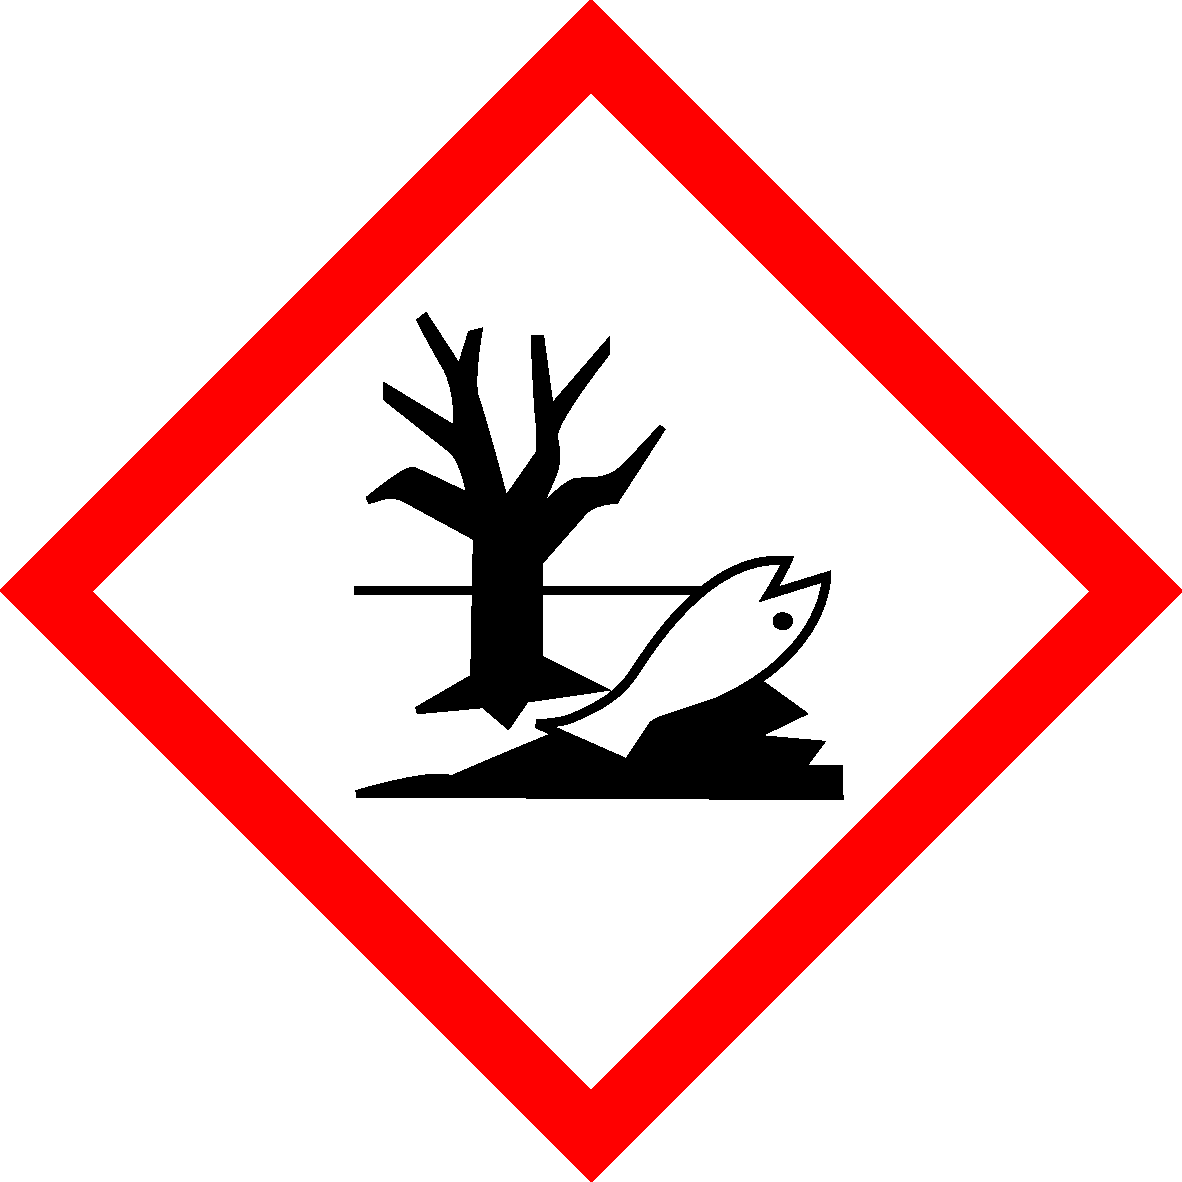
\includegraphics[height=24pt,valign=t]{pictos/envi.pdf} &  
H312, H315, H319, H335, H372, H400\newline P261, P273, P280, P305 + P351 + P338, P314\\
\midrule
Iodure de potassium\newline (7681-11-0, 166,00 g/mol) & 
\includegraphics[height=24pt,valign=t]{pictos/exclam.pdf} &  
H302, H315, H319\newline P305 + P351 + P338\\
\midrule
Rouge de méthyle, Solution\newline (269,3 g/mol) & 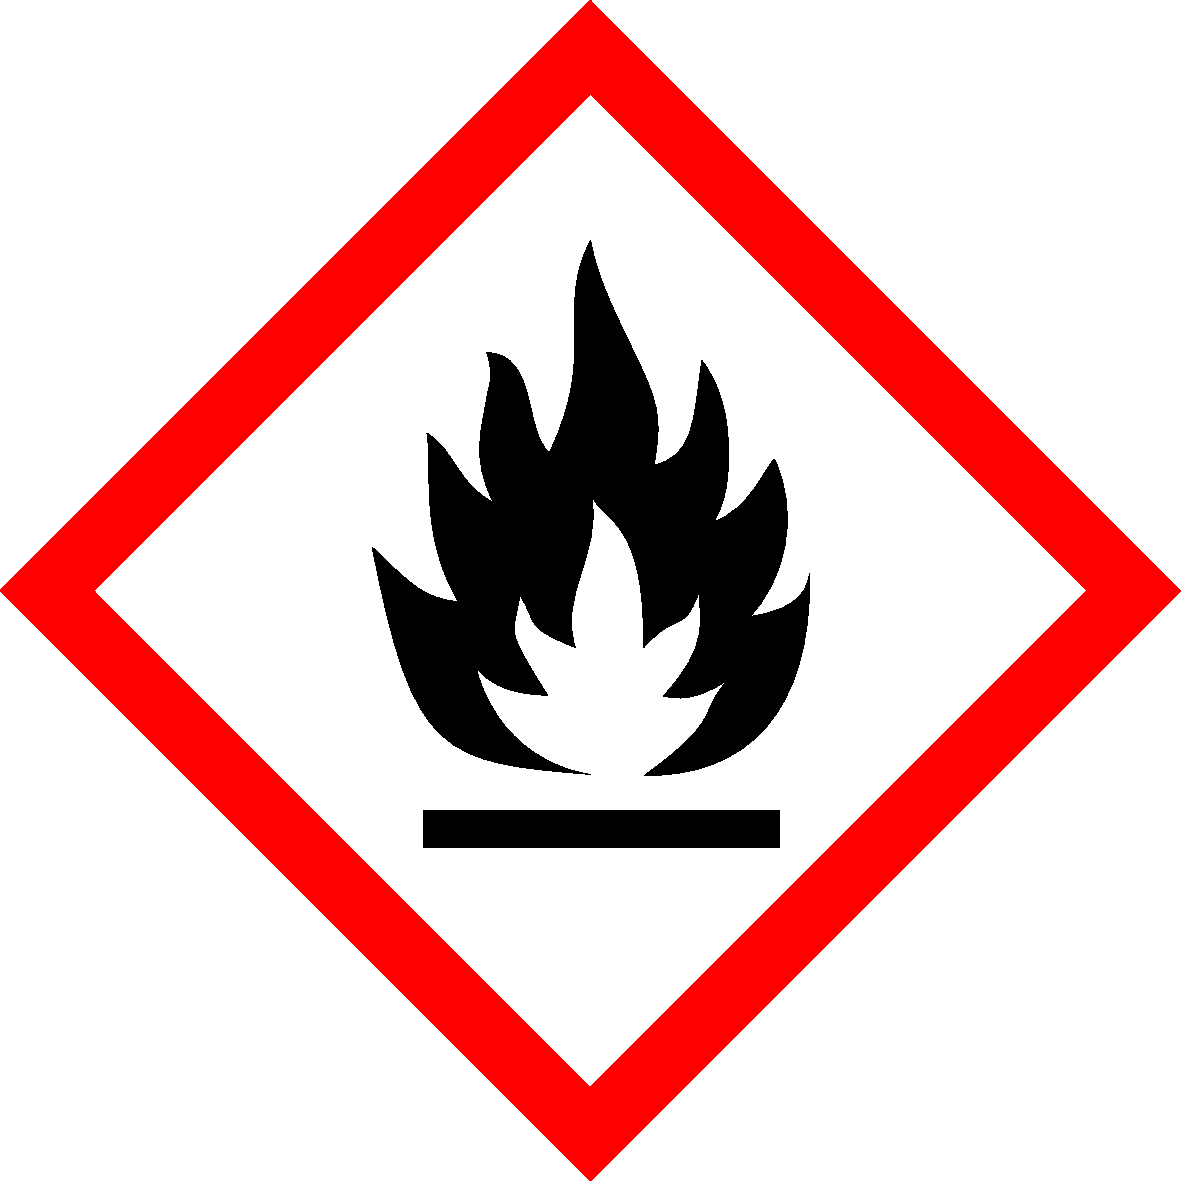
\includegraphics[height=24pt,valign=t]{pictos/flamm.pdf}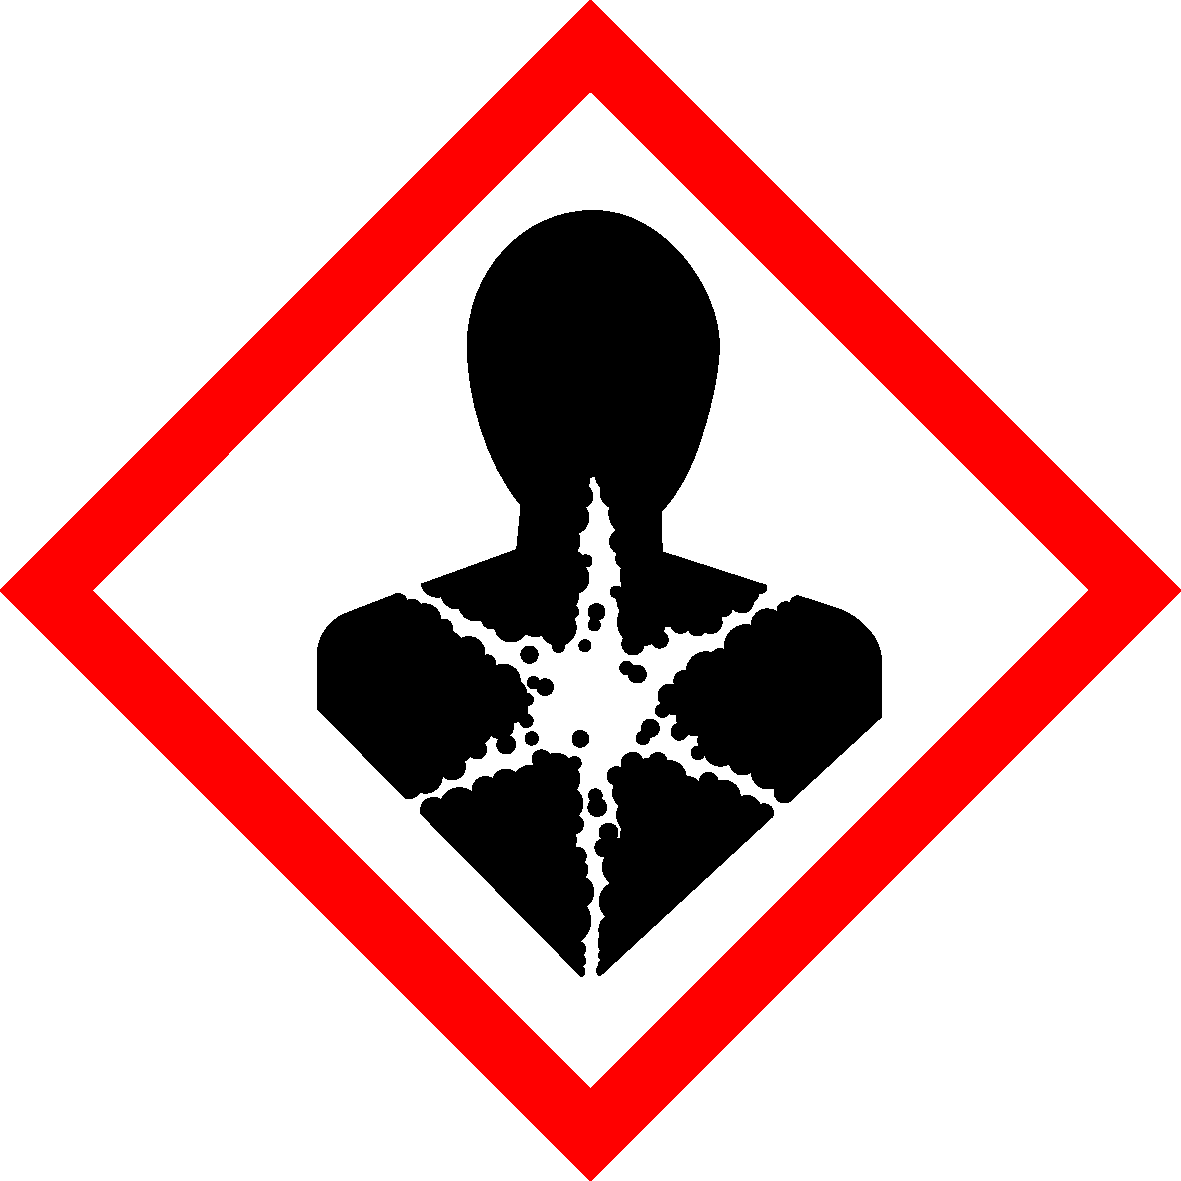
\includegraphics[height=24pt,valign=t]{pictos/cmr.pdf} 
\includegraphics[height=24pt,valign=t]{pictos/exclam.pdf} &  
H225, H319, H371\newline P210, P260, P280, P308 + P311, P337 + P313, P403 + P235\\
\midrule
Hydrochloric acid solution\newline (7647-01-0, 36,46 g/mol) & 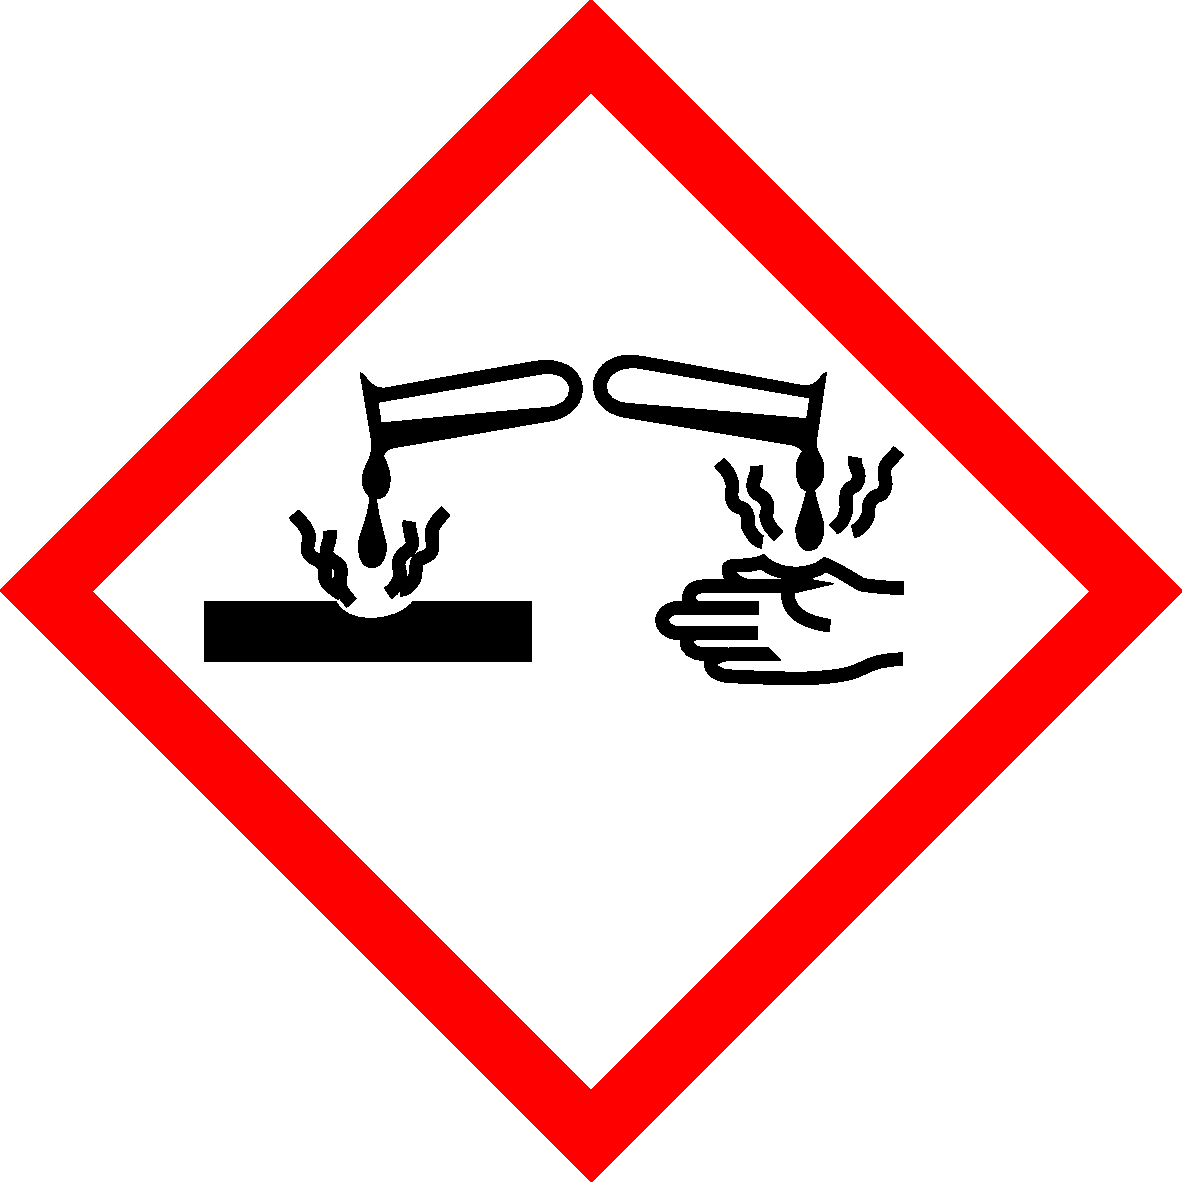
\includegraphics[height=24pt,valign=t]{pictos/corro.pdf} &  
H290 \\
\midrule
Acide sulfurique 20\% & 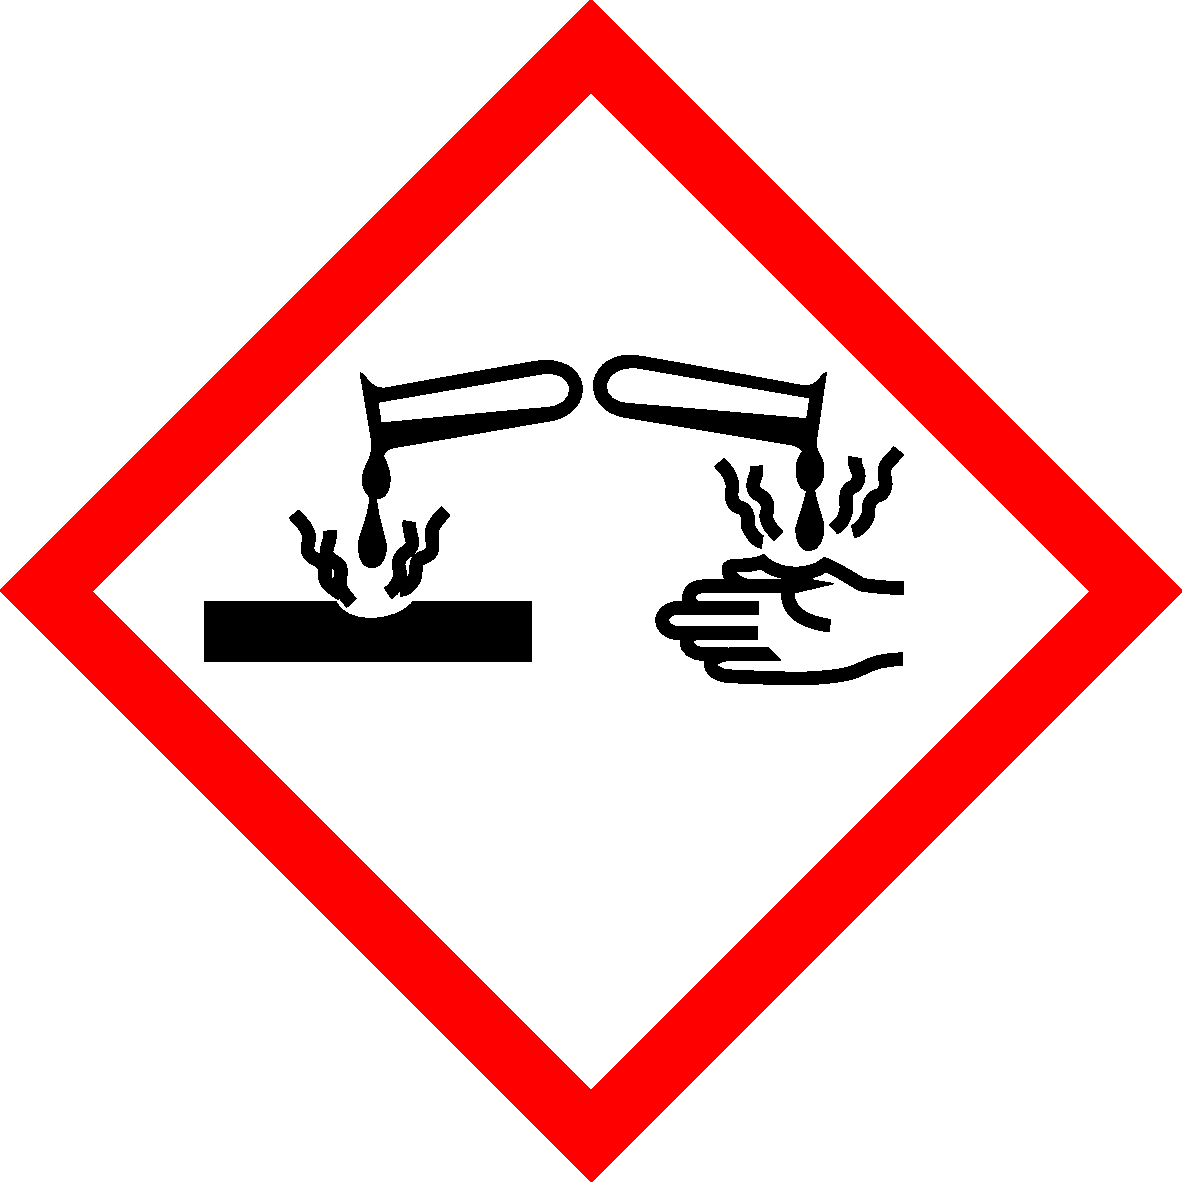
\includegraphics[height=24pt,valign=t]{pictos/corro.pdf} &  H314, H318, H401 \newline
P260, P264, P273, P280, P301 + P330 + P331, P303 + P361 + P353, P304 + P340, P305 + P351 + P338, P310, P363, P405, P501\\
\midrule
Éthanol\newline (64-17-5, 46,07 g/mol) & 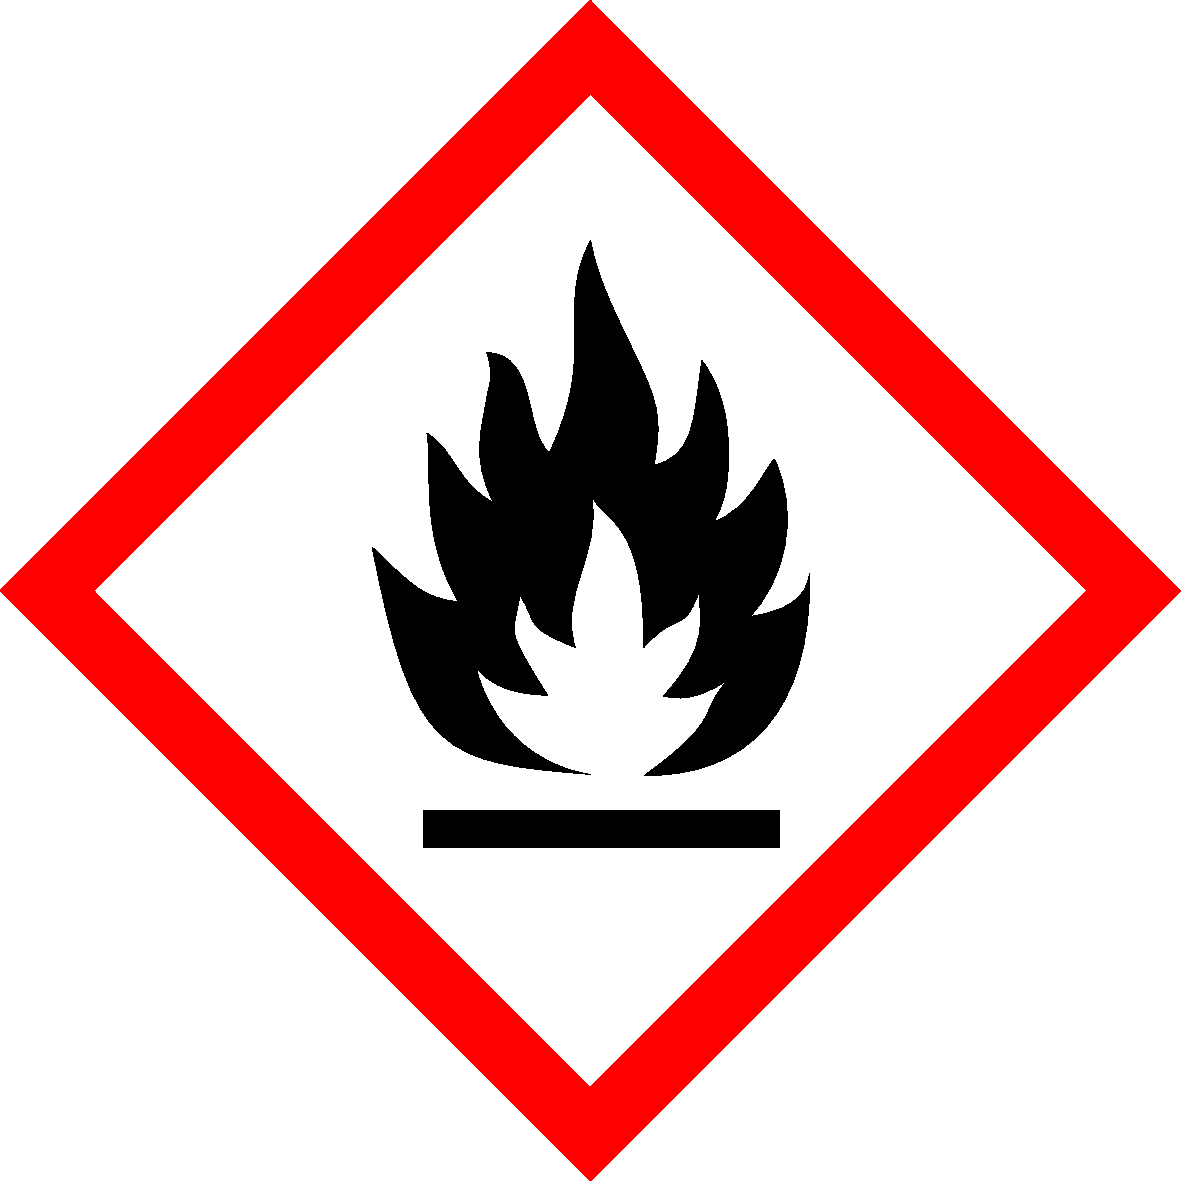
\includegraphics[height=24pt,valign=t]{pictos/flamm.pdf}
\includegraphics[height=24pt,valign=t]{pictos/exclam.pdf} &  
H225, H319\newline P210, P280, P305 + P351 + P338, P337 + P313, P403 + P235\\
\midrule
Acétate d'éthyle\newline (141-78-6, 88,11 g/mol) & 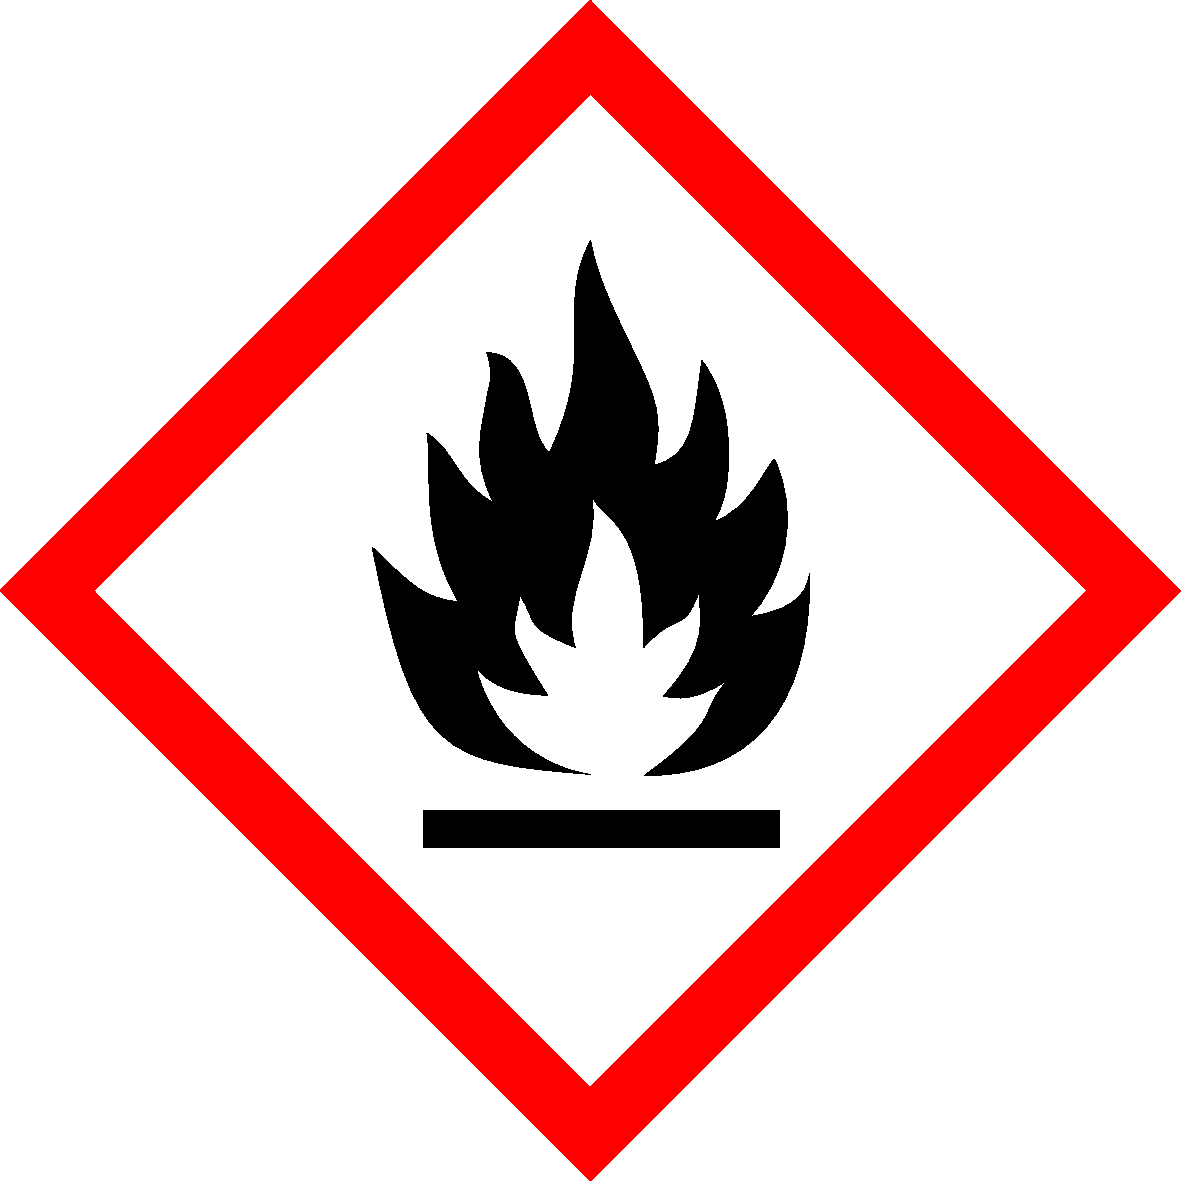
\includegraphics[height=24pt,valign=t]{pictos/flamm.pdf}
\includegraphics[height=24pt,valign=t]{pictos/exclam.pdf} &  
H225, H319, H336\newline P210, P305 + P351 + P338, P370 + P378, P403 + P235\\
\midrule
Sodium thiosulfate\newline (7772-98-7, 158,11 g/mol) &  &                                               \\  

\bottomrule
\end{tabular}



\end{document}
